\scanpage{141}
Papier brouillon (pour \unsure{Jordano|Jordens} ?)

\diagram{\begin{tikzcd}[ampersand replacement=\&]
\unsure{\mathscr J|J}\arrow[r,"\text{cof. ?}"]\arrow[dr,dashed]\&\mathscr J^B\arrow[d,"\text{cof ?}"]\\
I\arrow[u,"\text{cof}","{\text{pl fid}}"']\arrow[r,"\text{cof}"]\&I^B
\end{tikzcd}}
\margin{4.\unsure{9|4}.6.3. 2° p. \unsure{284--285|224--225}}

\[
\begin{aligned}
 &J\hookrightarrow I\\
 &\text{pl fid. cofinal}\qquad &\unsure{\not\Longrightarrow|\longmapsto}\quad J\ \text{grand devant }\pi\\
 &I\ \text{grand devant }\pi &&\text{OK}\ \unsure{\text{pour}}.
\end{aligned}
\]
\[
 \unsure{i|1}\rightrightarrows f(j)\longrightarrow\unsure{j'|y'}\longrightarrow f(j')
\]
\[
 \mathop{\mathrm{Card}}\alpha_0\leq\pi
\]
\[
 \deleted{J_0\quad J_1\quad J_2\quad\unsure{\cdots}\quad J_{\alpha}}
\]
\[
 J=\mathscr J_1\cap J_2\qquad\deleted{\unsure{\bigcap}}\quad\deleted{\unsure{J_\alpha}}
\]
$\operatorname{card} A=\unsure{\lambda^{\leq\pi}|\lambda\leq\pi}$ ($\alpha_\lambda$ plus petit ordinal de \unsure{cardinal} \unsure{$\lambda|\alpha$})

\figure{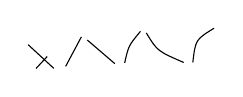
\begin{tikzpicture}[scale=.5]
\draw (0,.6)--(.65,0); \draw (.2,0)--(.48,.3); \draw (.95,.05)--(1.35,.8);
\draw (1.5,.72)--(2.2,.12); \draw (2.45,.14)..controls(2.55,.58)..(2.85,.94);
\draw (3,.9)..controls(3.28,.44)..(3.95,.15); \draw (4.18,.15)..controls(4.25,.73)..(4.72,1.02);
\end{tikzpicture}}
\[
 \operatorname{card}A\leq\pi
\]
$\alpha_0$ premier ordinal de cardinal \deleted{\unsure{$\leq$}} $\pi$

$I_{\alpha_0}\longrightarrow A$ tel que pour tt \deleted{\unsure{surjectif}} $r\in A$, $\varphi^{-1}(r)$ cofinal dans $\unsure{\mathbb I|I}_{\alpha_0}$ \unsure{i.e.|ou} $\operatorname{card}\varphi^{-1}(r)=\pi$
% archive sheet number: 141
